% the prelude is where package imports and some basic setup are performed
\documentclass[10pt, letterpaper, twocolumn]{article}

\usepackage{amsmath,amssymb,amsfonts}
\usepackage{graphicx}
\usepackage{fancyhdr}

\setlength{\topmargin}{-.5in} \setlength{\textheight}{9.25in}
\setlength{\oddsidemargin}{0in} \setlength{\textwidth}{6.8in}

\usepackage[sorting=none]{biblatex}
\usepackage[margin=1in,bottom=1.5in]{geometry}  % Adjust the bottom margin
\usepackage{graphicx}
\usepackage{changepage}
\usepackage{biblatex}
\usepackage{physics}
\usepackage{enumitem}
\usepackage{listings}
\usepackage{color}
\usepackage{cancel}

%++++++++++++++++++++++++++++++++++++++++

\setlength{\footskip}{1in}  % Adjust the footskip value

% we need fancy page style to have the footers
\pagestyle{fancy}

% if you need citations. otherwise, you can remove it
\addbibresource{citations.bib}

% document metadata goes here
\begin{document}
\title{Very Evil AP Exam}
\author{Richard M. Stallman}
\date{\today}
\maketitle

% the footer is added here. edit src/footer.tex to customize it, or
% remove it if you don't need it.
% this section controls the headers and footers on the first
% page
\fancypagestyle{plain}{
  \fancyhf{}
  \rfoot{\sffamily\bfseries\large{GO ON TO THE NEXT PAGE}}
  \cfoot{-~\thepage~-}
  \rhead{\large{Name: \underline{\hspace{3in}}}}
  % delete the header line
  \renewcommand{\headrulewidth}{0pt} 

% create the box around text in the bottom left
  \lfoot{
    \begin{minipage}[b]{\textwidth}
      \fbox{
        \begin{minipage}[b]{0.3\textwidth}
          \centering
          \sffamily\bfseries\footnotesize{Unauthorized copying or reuse of any part of this page is illegal.}
        \end{minipage}
      }
    \end{minipage}
  }
}

% this section controls the header and footer on every page that
% ISN'T the first or last page
\rfoot{\sffamily\bfseries\large{GO ON TO THE NEXT PAGE}}
\cfoot{-~\thepage~-}
% delete the header line
\renewcommand{\headrulewidth}{0pt} 

% create the box around text in the bottom left
\lfoot{
  \begin{minipage}[b]{\textwidth}
    \fbox{
      \begin{minipage}[b]{0.3\textwidth}
        \centering
        \sffamily\bfseries\footnotesize{Unauthorized copying or reuse of any part of this page is illegal.}
      \end{minipage}
    }
  \end{minipage}
}

% NOTE: the footer on the last page is defined in its own file (end.tex)

% Define a new page style for the last page
% \fancypagestyle{lastpage}{
%   \fancyhf{}
%   \rfoot{none}
% }


% here's where the MCQ questions are rendered. you can edit them in
% src/mcq.tex
\noindent{\bf Directions:}
Circle the best answer.

\large

\newcommand{\columnbreak}{{\par\vfill\null\pagebreak[4]}}

% the \columnbreak macro is provided to easily skip to the next column

\medskip\hrule
\begin{enumerate}
  \item Wrap both sides of Taylor's rule with the exponential function;
        then, compute the Taylor's Series of $e^{ix}$ centered at $x=\pi^*$
        and create a polynomial expansion with 4 terms for $e^i$. This
        polynomial expansion can best be expressed by which of the following
        expressions?
        \begin{enumerate}
          \item $\displaystyle \sum_{n=0}^{\infty} (-1)^n \dfrac{x^n}{n!}$
          \item $\displaystyle \MultiIntegral{3} x^3 e^x \differential x$
          \item $e^{2 \pi i k} - e^{2 \pi i (k + 1)}$
          \item $\displaystyle\sum_{n=-\infty}^{\infty} a_n \int_\gamma (z - z_0)^n \differential z$
        \end{enumerate}


  \item In order for Goldman Sachs to most effectively launder
        Malaysia's \textsc{1MDB} sovereign wealth fund, what economic policy
        would be best?
        \begin{enumerate}
          \item Lower the reserve requirement for foreign banks
          \item Increase the reserve requirement for foreign banks
          \item Lower the reserve requirement for domestic banks
          \item Increase the reserve requirement for domestic banks
        \end{enumerate}

  \item If Biden authorizes a \textsc{SWIFT} international banking
        transaction to launder money from Burisma in Ukraine to a hedge
        fund in Washington, D.C., it is an example of which of the
        following types of governmental economic involvement?
        \begin{enumerate}
          \item Open-market operations
          \item Reserve ratio
          \item Discount rate
          \item Government spending
        \end{enumerate}


        % you can also add context to a problem, like this:
        \vspace{0.5cm}

        In 2020, researchers at the University of California, Berkeley
        developed a new margin-based Condorcet voting algorithm called
        Split Cycle, which avoids common pitfalls associated with
        Condorcet voting methods such as ``spoiler effects'' and
        ``strong no show paradoxes''~\cite{splitcycle}.

        \bigskip

        \begin{figure}[h]
          \centering
          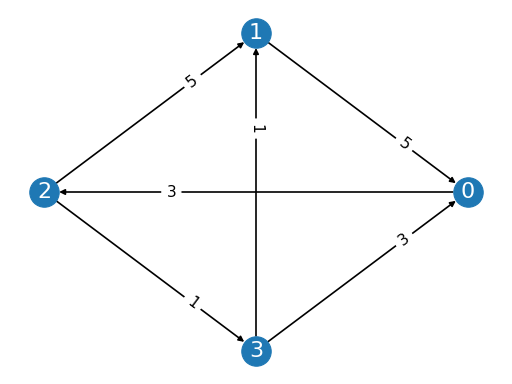
\includegraphics[width=0.4\textwidth]{assets/splitcycle.png}
          \label{}
          \caption{Voting margins graph}
        \end{figure}

  \item Consider the voting margins matrix above.
        % Define colors for Python syntax highlighting
\definecolor{codegreen}{rgb}{0,0.6,0}
\definecolor{codegray}{rgb}{0.5,0.5,0.5}
\definecolor{codepurple}{rgb}{0.58,0,0.82}
\definecolor{backcolour}{rgb}{0.95,0.95,0.92}

% Define Python language settings
\lstdefinestyle{pythonstyle}{
  backgroundcolor=\color{backcolour},
  commentstyle=\color{codegreen},
  keywordstyle=\color{magenta},
  numberstyle=\tiny\color{codegray},
  stringstyle=\color{codepurple},
  basicstyle=\ttfamily\footnotesize,
  breakatwhitespace=false,
  breaklines=true,
  captionpos=b,
  keepspaces=true,
  numbers=left,
  numbersep=5pt,
  showspaces=false,
  showstringspaces=false,
  showtabs=false,
  tabsize=2
}

\lstset{style=pythonstyle}

\begin{lstlisting}[language=Python, caption=Calling Split Cycle from Python]
from pref_voting.margin_based_methods import split_cycle

split_cycle.display(mg)
\end{lstlisting}


        The above code will run the split cycle algorithm on the margin
        graph. Who will the Condorcet winners be?

        \begin{enumerate}
          \item $\begin{Bmatrix} 2 & 3 \end{Bmatrix}$
          \item $\begin{Bmatrix} 0 & 2 \end{Bmatrix}$
          \item $\begin{Bmatrix} 1 & 3 \end{Bmatrix}$
          \item $\begin{Bmatrix} 2 & 1 \end{Bmatrix}$
        \end{enumerate}
\end{enumerate}


\onecolumn

% set time for the FRQ here
\begin{adjustwidth}{1in}{1in}
  \begin{center}
    \textbf{
      CHAPTER 14 \\
      \medskip
      SECTION II: FREE RESPONSE \\
      \medskip
      Total Time -- 15 minutes \\
      \medskip
      Reading Period -- 5 minutes \\
      \medskip
      Writing Period -- 10 minutes}
  \end{center}
\end{adjustwidth}

% here's where the FRQ questions gets rendered. you can edit it in the
% src/frq.tex file
\bigskip
\noindent\textbf{Directions}: You are advised to spend the first 5 minutes
reading all of the questions and planning your answers. You will then
have 10 minutes to answer all three of the following questions. You may
begin writing your responses before the reading period is over. It is
suggested that you spend approximately half your time on the first
question and divide the remaining time equally between the next two
questions. Include correctly labeled diagrams, if useful or required, in
explaining your answers. A correctly labeled diagram must have all axes
and curves clearly labeled and must show directional changes. If the
question prompts you to “Calculate,” you must show how you arrived at
your final answer. Use a pen with black or dark blue ink. \\

\clearpage

% add content below.

\begin{enumerate}[itemsep=0.5cm]
      \item
            \begin{figure}[h]
                  \centering
                  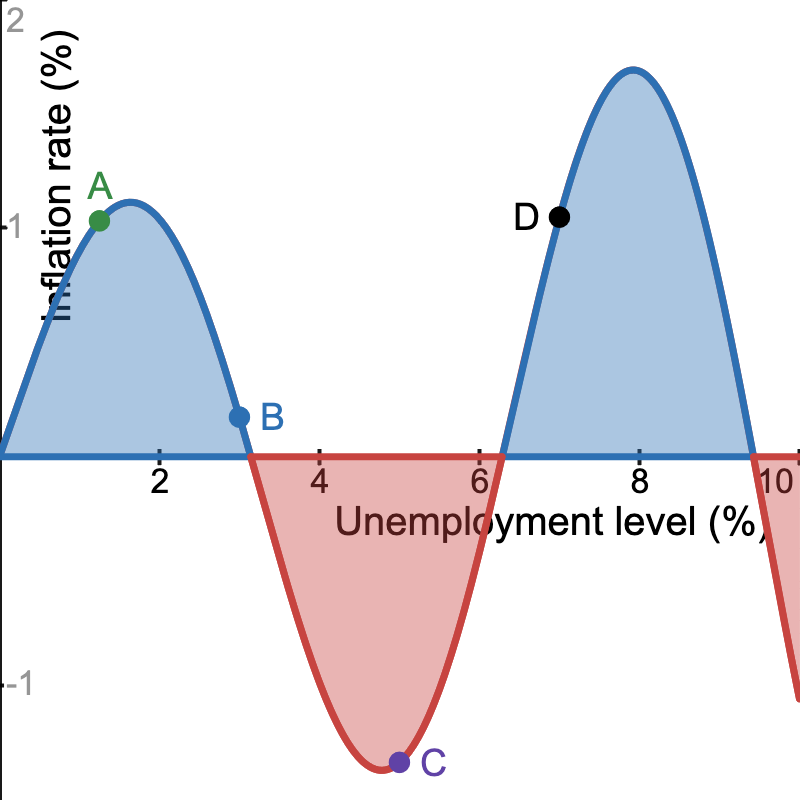
\includegraphics[width=0.4\textwidth]{assets/phillips.png}
            \end{figure}

            \[
                  f\left(x\right)=\sin\left(x\right)e^{x/15}
            \]

            At a campaign event, Barack Obama was confronted with a voter
            named Joe who was unemployed and complaining about rampant
            inflation during the Obama regime. Joe claimed that he was
            paying too much tax and became a martyr among conservative
            circles, known as ``Joe the Plumber'' (RIP). \\
            \medskip

            Consider the above graph, which represents the Phillips Curve
            during Obama's 2-term presidency. Answer the following questions:\@

            \bigskip

            \begin{adjustwidth}{0.3in}{0.3in}
                  \begin{enumerate}[itemsep=0.5cm]

                        % integral represents misery index
                        % point b maximizes misery index
                        \item Identify the point on the Phillips curve that best
                              corresponds to Obama's fiscal policy, assuming that
                              what Joe is saying is correct and assuming that Joe
                              represents the average American.
                        \item Identify the central relationship between inflation
                              and unemployment that is the basis for the Philips Curve.

                        \item This is only nominally a Phillips curve,
                              since it doesn't assume that unemployment
                              and inflation have an inverse
                              relationship. Extrapolate this information
                              to determine whether the Phillips curve's
                              hypothesis still holds true in the modern
                              age.

                              \clearpage

                        \item
                              In the 1970s, Arthur Okun, economic adviser to
                              President Lyndon B. Johnson, proposed the ``Misery
                              Index'' as an indicator of economic
                              health~\cite{inflationdata}. It's defined as
                              $Unemployment\,Rate \times Inflation\,Rate$

                              \begin{enumerate}
                                    \item If we were to evaluate $\displaystyle \int f(x) \,
                                                \differential x$, what would it represent?

                                    \item Develop a strategy for evaluating the misery
                                          index at a point using the Taylor Series
                                          approximation of $f(x)$. What Maclaurin series do
                                          you need to manipulate to develop a Taylor series
                                          approximation for $f(x)$?

                                    \item Use the Taylor remainder theorem to determine
                                          how many terms you need to add or multiply in order
                                          to ensure that your estimation of the misery index
                                          is accurate to within two decimal places.

                                    \item Identify the point ($A$, $B$, $C$, or
                                          $D$) on the graph which maximizes the misery
                                          index.
                              \end{enumerate}
                        \item Assume that Joe's complaints are valid. Determine null
                              and alternate hypotheses relating to the inflation rate
                              given what we know about Joe's situation.

                        \item Given a random sample of $n$ Americans, $p$ percentage
                              of them agree with Joe's assumptions. At what value of
                              $p$ can we conclude that there is a statistically
                              significant reason to reject the null hypothesis $H_0$
                              (at the $\alpha = 0.05$ confidence level)?

                        \item Interpret your conclusions from parts (f) and (d) and
                              state the result. With what confidence and accuracy can we
                              assess the misery index?

                        \item Identify the potential consequences of a Type I error
                              in this scenario and what can be done, if anything, to
                              resolve it. What about a Type II error?
                  \end{enumerate}
            \end{adjustwidth}
\end{enumerate}


% here's where the final page with the STOP sign is rendered
% you can remove it, or edit src/end.tex to customize it
\onecolumn
\sffamily
\bfseries
\begin{adjustwidth}{1in}{1in}
  \begin{center}
    \begin{figure}[h]
      \centering
      
\includegraphics[width=0.4\textwidth]{assets/stop.jpg}
      \label{}
    \end{figure}
    \Large
    END OF EXAM \\
    \bigskip
    IF YOU FINISH BEFORE TIME IS CALLED, YOU MAY
    CHECK YOUR WORK ON THIS SECTION\@
  \end{center}
\end{adjustwidth}



\large

% remove this bibliography section if you don't need it
% \printbibliography

\end{document}
